 \documentclass[a4paper,9pt]{beamer}\usepackage[]{graphicx}\usepackage[]{color}
% maxwidth is the original width if it is less than linewidth
% otherwise use linewidth (to make sure the graphics do not exceed the margin)
\makeatletter
\def\maxwidth{ %
  \ifdim\Gin@nat@width>\linewidth
    \linewidth
  \else
    \Gin@nat@width
  \fi
}
\makeatother

\definecolor{fgcolor}{rgb}{0.345, 0.345, 0.345}
\newcommand{\hlnum}[1]{\textcolor[rgb]{0.686,0.059,0.569}{#1}}%
\newcommand{\hlstr}[1]{\textcolor[rgb]{0.192,0.494,0.8}{#1}}%
\newcommand{\hlcom}[1]{\textcolor[rgb]{0.678,0.584,0.686}{\textit{#1}}}%
\newcommand{\hlopt}[1]{\textcolor[rgb]{0,0,0}{#1}}%
\newcommand{\hlstd}[1]{\textcolor[rgb]{0.345,0.345,0.345}{#1}}%
\newcommand{\hlkwa}[1]{\textcolor[rgb]{0.161,0.373,0.58}{\textbf{#1}}}%
\newcommand{\hlkwb}[1]{\textcolor[rgb]{0.69,0.353,0.396}{#1}}%
\newcommand{\hlkwc}[1]{\textcolor[rgb]{0.333,0.667,0.333}{#1}}%
\newcommand{\hlkwd}[1]{\textcolor[rgb]{0.737,0.353,0.396}{\textbf{#1}}}%
\let\hlipl\hlkwb

\usepackage{framed}
\makeatletter
\newenvironment{kframe}{%
 \def\at@end@of@kframe{}%
 \ifinner\ifhmode%
  \def\at@end@of@kframe{\end{minipage}}%
  \begin{minipage}{\columnwidth}%
 \fi\fi%
 \def\FrameCommand##1{\hskip\@totalleftmargin \hskip-\fboxsep
 \colorbox{shadecolor}{##1}\hskip-\fboxsep
     % There is no \\@totalrightmargin, so:
     \hskip-\linewidth \hskip-\@totalleftmargin \hskip\columnwidth}%
 \MakeFramed {\advance\hsize-\width
   \@totalleftmargin\z@ \linewidth\hsize
   \@setminipage}}%
 {\par\unskip\endMakeFramed%
 \at@end@of@kframe}
\makeatother

\definecolor{shadecolor}{rgb}{.97, .97, .97}
\definecolor{messagecolor}{rgb}{0, 0, 0}
\definecolor{warningcolor}{rgb}{1, 0, 1}
\definecolor{errorcolor}{rgb}{1, 0, 0}
\newenvironment{knitrout}{}{} % an empty environment to be redefined in TeX

\usepackage{alltt}
 
 \mode<presentation>
{
  \usetheme{Singapore}      % or try Darmstadt, Madrid, Warsaw, ...
  \usecolortheme{} % or try albatross, beaver, crane, ...
  %\usefonttheme{serif}  % or try serif, structurebold, ...
  \mode<presentation>{\useinnertheme{rounded}}
  \setbeamertemplate{navigation symbols}{}
  \setbeamertemplate{caption}[numbered]
  \addtobeamertemplate{navigation symbols}{}{%
    \usebeamerfont{footline}%
    \usebeamercolor[fg]{footline}%
    \hspace{1em}%
    %\insertfrawas done by one doctor menumber/\inserttotalframenumber
}
} 

\usepackage{tikz}
\usepackage{float}
\usepackage{graphicx}
\usepackage{mathtools}
\usepackage{amsmath}
\usepackage[english]{babel}
\usepackage[utf8x]{inputenc}
\usepackage{color, colortbl}
\usepackage{subfig}
\usepackage{listings}
%\usepackage[style=authoryear]{biblatex}
%\usepackage[latin1]{inputenc}
\usefonttheme{professionalfonts}
\usepackage{times}
%\usepackage{tikz}
%\usetikzlibrary{arrows,shapes}
%\usepackage[colorlinks,citecolor=red,linkcolor=black]{hyperref}
\usepackage[super,comma,sort&compress]{natbib}
   \bibliographystyle{apalike}
    \usepackage{float}
    %\usepackage[utf8]{inputenc}
    %\usepackage[style=numeric]{biblatex}
    \usepackage[english]{babel}
    \usepackage{multicol}
    %\usepackage{dirtytalk}
%\usepackage{fancyhdr}

\title{Measuring intraspecific diversity: a critical assessment of methods}

\author{Olusoji O. D.$^{1, 2}$, Spaak J.$^{1}$, Neyens T.$^{2}$, Fontana S.$^{3}$, \\Aerts M.$^{2}$, De Laender F.$^{1}$}
\institute{Environmental and Evolutionary Biology (URBE), Univeriste De Namur, Belgium$^{1}$, \\Center for Statistics, Universiteit Hasselt, Belgium$^{2}$, \\Swiss Federal Institute for Forest, Snow and Landscape Research, Birmensdorf, Switzerland$^{3}$}\\

 %\textcolor{red}{ESAUSSE, LOUISVILLE 2019}
\titlegraphic{
\includegraphics[width=3.5cm,height=1.0cm,scale=0.7]{Ibiostat_logo.png} ~% 
\hspace*{0.75cm} 
\includegraphics[width=2cm,height=1.5cm,scale=0.7]{ilee.JPG}
\hspace*{0.75cm} 
\includegraphics[width=1.5cm,height=1.4cm,scale=0.1]{Unamur_logo.jpg}
  }

\date{August 13, 2019}

\beamertemplatenavigationsymbolsempty

%\setbeamerfont{page number in head/foot}{size=\large}
\setbeamertemplate{footline}[frame number]
\IfFileExists{upquote.sty}{\usepackage{upquote}}{}
\begin{document}
%\SweaveOpts{concordance=TRUE}
%\SweaveOpts{concordance=TRUE}

\frame{\maketitle}

\section{Intraspecific Diversity (ITD)}

\begin{frame}{Intraspecific Diversity, what is it?}

\begin{columns}

\begin{column}{0.5\textwidth}
\begin{block}{ITD Definition}

\begin{tikzpicture}
\draw (0,0) circle (3pt);
\end{tikzpicture} $-$ Species one, \begin{tikzpicture}
\draw (0,0) rectangle ++(4pt,4pt);
\end{tikzpicture} $-$ Species two
\vspace{-0.6cm}
\begin{knitrout}
\definecolor{shadecolor}{rgb}{0.969, 0.969, 0.969}\color{fgcolor}

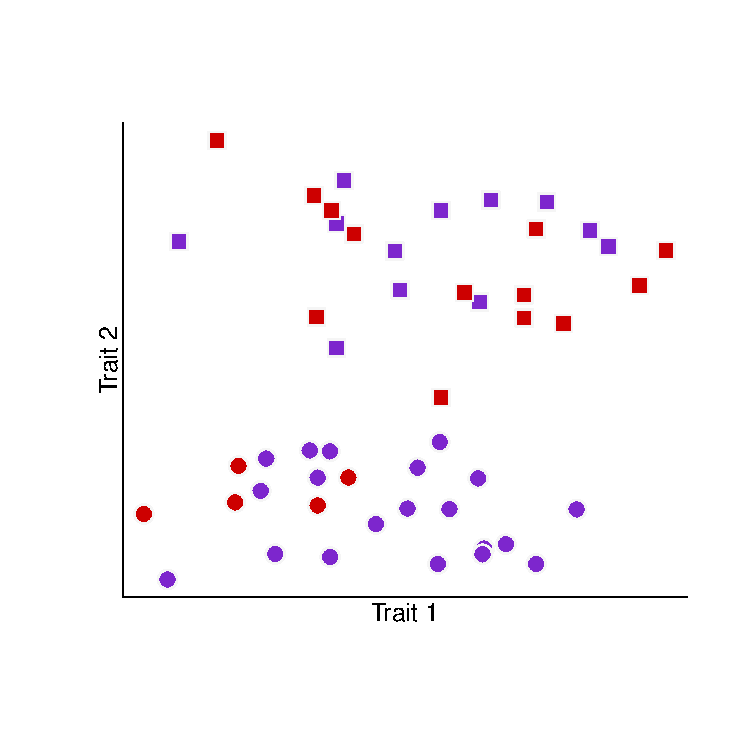
\includegraphics[width=\maxwidth]{figure/r_intra-1} \hfill{}



\end{knitrout}
\end{block}

\end{column}

\begin{column}{0.5\textwidth}
\uncover<2->{\begin{block}{Facets of Intraspecific Diversity}

\begin{itemize}
\item Richness(what amount of the trait space is occupied by individuals of the same species?)
\item Evenness(how is the trait space filled up by these individuals?)
\item Divergence(any form of trait differentiation across these individuals?)
\end{itemize}

\end{block}
}
\end{column}

\end{columns}

\end{frame}

\begin{frame}{How is Intraspecific Diversity Measured?}

\begin{itemize}
\item Via indices!
\item We concentrate on \alert{multi-trait indices}
\end{itemize}

\begin{columns}
\begin{column}{0.33\textwidth}

\begin{block}{Trait Richness}
\begin{itemize}
\item FRic (Villeger et al., 2008)
\item TOP (Fontana et al., 2016)
\end{itemize}
\end{block}

\end{column}

\begin{column}{0.33\textwidth}
\begin{block}{Trait Evenness}
\begin{itemize}
\item FEve (Villeger et al., 2008)
\item TED (Fontana et al., 2016)
\end{itemize}
\end{block}


\end{column}

\begin{column}{0.33\textwidth}
\begin{block}{Trait Divergence}
\begin{itemize}
\item Rao (Rao, 1982)
\item FDis (Lalibert \& Legendre, 2010)
\end{itemize}
\end{block}


\end{column}

\end{columns}

\end{frame}

\begin{frame}{Something New?}

\begin{columns}
\begin{column}{0.5\textwidth}
\begin{block}{Modified TED (TEDM)}

\end{block}
\end{column}

\begin{column}{0.5\textwidth}
\begin{block}{Modified TOP (TOPM)}

\end{block}

\end{column}

\end{columns}
\end{frame}

\section{ITD Criteria}

\begin{frame}{What to Expect from ITD Indices?}
Simone's criteria and our proposed additional criteria

\end{frame}


\section{Simulation and Results}

\begin{frame}{Simulation Framework}


\end{frame}

\begin{frame}{Results}


\end{frame}

\section{Take Away}

\begin{frame}{Conclusion}


\end{frame}



\end{document}
